\chapter{Physical Layer}

\section{Radio Signals}
Most of the wireless technology used today is based on radio frequency 
signals. 
Radio signals are electromagnetic energy generated by high frequency 
alternate current in antennas. They can have different frequencies and lengths 
and propagate differently depending on the medium they need to cross.

Radio frequencies have three main properties:
\begin{itemize}
\item \textbf{Amplitude}: determines how far a signal can 
  travel (remember that reaching 2x distance requires 4x power). It is the 
  difference between the highest and lowest wave peak.
\item \textbf{Frequency}: the number of oscillations in 1 second
\item \textbf{Wavelength}: the distance between two high (or low) peaks. The
  wavelength is $\frac{c}{frequency}$ and this means that, in practice, antennas
  work better with sizes 1, $\frac{1}{2}$, $\frac{1}{4}$ of wavelength.
\end{itemize}

\paragraph*{Propagation} From its origin, after a certain point the 
signal is no longer detectable. If there is an obstacle the signal loses power 
more quickly because obstacles can reflect or absorb waves depending on 
materials and waves frequencies.
When dealing with RF propagation we can rely on a rule of thumb: high 
frequencies are good for short distances and are affected by obstacles, while 
low frequencies are good for long distances and are less affected by obstacles.

RF have other properties that describe their behavior: they can phase, 
that is done shifting the wave (in degrees or radians) and are affected by the
physical orientation of the antenna (polarization).
Waves propagate in a toroid form (donut form).

The propagation range depends on power, obstacles, the receiver's 
sensitivity and many other factors. We have different ranges:
\begin{itemize}
\item \textbf{Transmission Range}: marks how far can the communication 
  reach;
\item \textbf{Detection Range}: marks how far the detection of the signal 
  is possible;
\item \textbf{Interference Range}: marks the distance at which the signal 
  is too far away from the sender to be detected and so it just adds to the 
  background noise.
\end{itemize}
Also, a lot of different \mKeyword{physical effects} can affect propagation, in 
particular: shadowing, reflection, refraction (happens when passing to a 
different medium), scattering (at a corner the power is sent in different 
directions), diffraction (splitting the signal in 2).
The final signal received could therefore be better or worse than the 
one originally sent, with signals taking different paths towards their 
destination. See Figure~\ref{fig:ewn:Propagation} to see the different effects 
of propagation.

\begin{figure}[h]
  \centering
  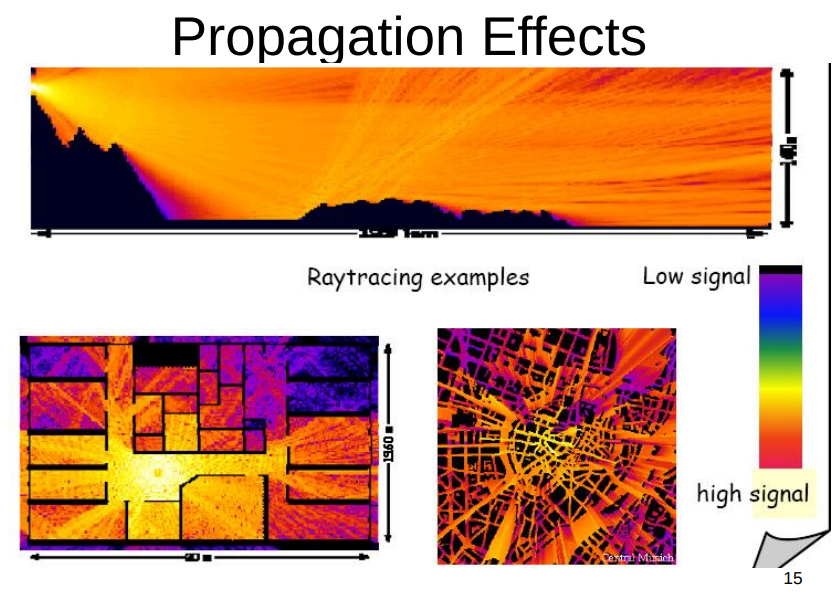
\includegraphics[width=0.8\linewidth]{Propagation.png}
  \caption{The different effects of propagation}
  \label{fig:ewn:Propagation}
\end{figure}

\section{Antennas}
Antennas convert energy in RF waves (transmission) and vice-versa 
(reception). As explained in the previous section, the size of antennas is 
related to the RF frequency of transmission and reception.
Starting from the simple dipole antenna, we can have different types of 
antennas.

\subsection{Omnidirectional Antennas}
\begin{figure}[t]
  \centering
  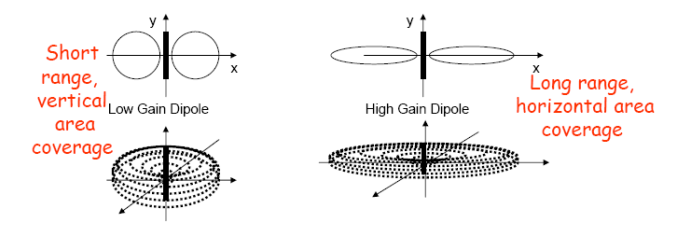
\includegraphics[width=0.8\linewidth]{OmnAnt.png}
  \caption{Omnidirectional Antennas}				
  \label{fig:ewn:OmnAnt}
\end{figure}
They radiate RF power equally in all directions around the vertical axis, the
most common example is the dipole antenna. They can cover both short and long
range.
Near and below the dipole the signal is weak, a better radiation is 
obtained in sub-areas around the dipole. An omnidirectional antenna is better 
suited when there is a need for uniform radio coverage around a central point. 
Outdoors, it can be used for point-to-multipoint connections (star topology). 
Note that the tilt of the antenna changes the position of the y axis and can be 
exploited to reach computers on different floors.

\subsection{Semi-directional Antennas} They don't transmit in all 
directions and can be positioned against walls without wasting too much signal. 
Some types are Patch/panel and Yagi.

\subsection{Highly-directional Antennas} They are used by parabolic 
dishes and grids. They reach very far, covering a distance of up to 60 km 
assuming no obstacles in-between (LOS=Line Of Sight). Putting the sender and the 
receiver too far away causes the signal to hump against the curve of the Earth. 
Highly-directional Antennas need to be placed carefully, for the signal to be 
received they have to be perfectly aligned and prevent wind or bad weather from 
tilting them.
Another important point to consider is the \mKeyword{\textbf{Fresnel Zone}}:
when transmitting, the power isn't all concentrated in the center and it doesn't
actually proceed in a straight line.

\begin{figure}[h]
  \centering
  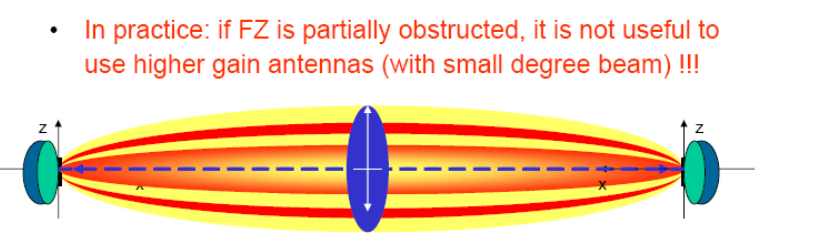
\includegraphics[width=0.8\linewidth]{Fresnel.png}
  \caption[The Fresnel Zone]{The Fresnel Zone: the red areas represent
    high-energy areas of the signal}				
  \label{fig:ewn:Fresnel}
\end{figure}

We have to be aware of this fact and check that there are no obstacles 
blocking the external high-energy areas (that end up carrying most of the 
signal!).
The diameter of the Fresnel Zone depends on 2 parameters:
\begin{itemize}
\item Distance
\item Frequency
\end{itemize}
So it is independent from the energy used.

\section{Wireless Spectrum}
Wireless uses a dedicated area of the spectrum. See
Figure~\ref{fig:ewn:WLSpectrum} for a breakdown of the wireless spectrum.

\begin{figure}[h]
  \centering
  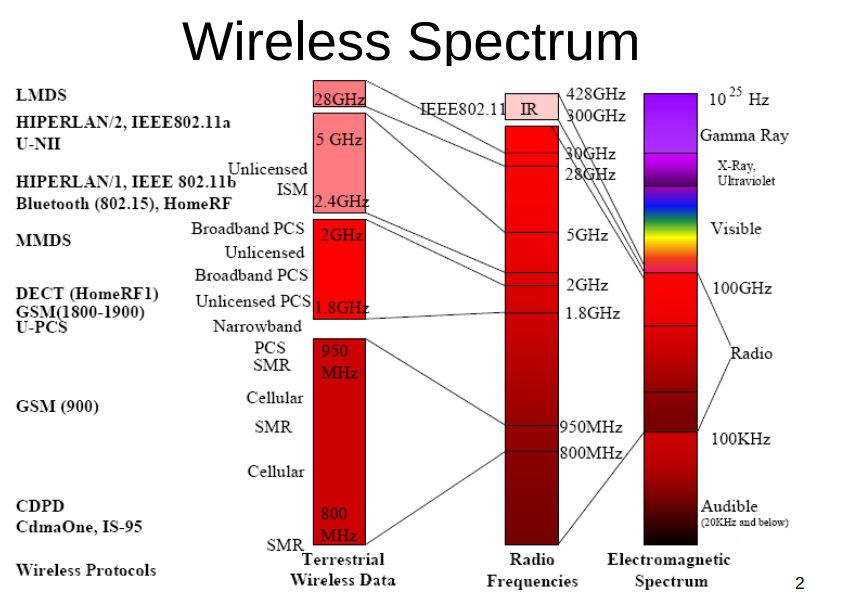
\includegraphics[width=0.8\linewidth]{WLSpectrum.png}
  \caption{The wireless spectrum}				
  \label{fig:ewn:WLSpectrum}
\end{figure}	

How can wireless channels have different bandwidth (BW)? We can't make 
bits move faster, they already travel at the speed of light. But, instead, we 
can think of sending them faster (more frequently, they travel at the same 
speed but are more packed).
Two nodes that need to exchange information need to be in each other's 
radio transmission coverage radius. Depending on the transmission power of the 
nodes we can have different situations:
\begin{itemize}
\item Unidirectional Link: sometimes improperly referred as 
  ``asymmetric link'' (we have an asymmetric link if A transmits at 10Mb/s while
  B transmits at 2Mb/s), we have a unidirectional link if, given A and B, A
  receives B but B cannot receive A. This is the case, for example, when B is
  just broadcasting or flooding the channel. Note that with a unidirectional
  link we can't share a file between A and B: B will be waiting for an ACK that
  never comes.
\item Bidirectional Link: A receives B and B receives A. It can be both:
 \begin{itemize}
 	\item symmetric: all devices send at the same speed;
 	\item asymmetric: different speed of transmission between devices in the
  network.
 \end{itemize}
\end{itemize}

\section{Examples of wireless network technology}

\subsection{Frequency Hopping Spread Spectrum}
To make a better use of the whole band, we can divide it in smaller frequencies.
The sender and the receiver will know the jump sequence and transmit in a
``secret'' pattern, to others this will appear as impulse noise and so the
communication will be more difficult to detect. Because of the continuous
hopping, it has a low throughput.

\subsection{Infrared Technology (IR)}
Requires short rage and line of 
sight (LOS). It uses frequencies just below the visible light and cannot 
penetrate opaque objects. It has a high bandwidth.

\section{Wireless Network Coverage}
We have different names for wireless technology depending on their 
coverage:
\begin{itemize}
\item Wireless Wide Area Network (WWAN): it covers large 
  geographical areas, like countries or regions;
\item Wireless Metropolitan Area Network (WMAN): metropolitan 
  coverage;
\item Wireless Local Area Network (WLAN): used for local area 
  coverage, like campuses,  and buildings (even the one commonly used at home);
\item Wireless Personal Areal Network (WPAN): reduced area 
  coverage, for example Bluetooth, houses are already too much;
\item Wireless Indoor Area Network (indoor): really short 
  coverage.
\end{itemize}

Note that, even in wireless connections, access points need to have both 
the wired and wireless protocols because they don't just relay the information, 
they have to translate it.

\section{Multiplexing}
The goal of multiplexing is to have different channel that can share the same
medium using different dimensions. These dimensions are:
\begin{itemize}
\item space;
\item time: user uses one channel for a certain amount of time. This technique
  requires synchronization;
\item frequency: spectrum is divided into smaller frequency bands. A certain
  band is given all the time to one single channel. May be a waste of bandwidth
  if use of channel are unbalanced;
\item code: all channels use the same spectrum but speak a different language.
  Data of channels is blob together but can be decode thank to the different
  code assigned to channels.
\end{itemize}

